\chapter{Footprint}
\label{chap:fp}

In this chapter, we investigate the difficulty of measuring footprint
completely and efficiently. Previous techniques either profile
only a small subset of windows to guarantee measurement efficiency or profile all
windows with impractical overhead. We propose two techniques, all-footprint
analysis and average-footprint analysis, to overcome the
challenge. These two techniques improve the overhead of previous
all-window measurements drastically without sacrificing
measurement accuracy. To further reduce/hide measuring overhead and
make footprint an on-line measurable metrics, we apply shadow sampling
on average-footprint analysis. With all efforts introduced
later in the following sections, we are able to get all-window
footprint statistics for target programs, such as SPEC2000/SPEC2006
benchmark suites, with almost zero time cost.

The techniques introduced in this chapter serves as the foundation of
this dissertation. With full footprint information available, we are
able to build connections between footprint and other locality
metrics(Chapter~\ref{chap:model}), set up footprint based cache
sharing models(Chapter~\ref{chap:corun}), and explore potentials of
footprint in various related fields.

\section{Introduction}
Many techniques are based on the notion of working set, which is
the volume of data accessed in a time window. The program working set is
known as the program footprint. Since program footprint shows active
data usage, it has been used to model resource sharing among
concurrent tasks, either in sharing memory among multiprogrammed
workloads or more recently in sharing cache among multicore workloads.
Various notions of working set and footprint have been studied extensively
for improving fairness and performance of concurrent executions
over shared cache and memory.

Let $n$ be the length of a trace and $m$ the number of distinct
data in the trace. A trace of $n$ data accesses has ${{n}\choose{2}} = \frac{n (n-1)}{2}$
distinct windows and therefore $\frac{n (n-1)}{2}$ footprints.
We consider so-called ``on-line'' profiling, which
traverses the trace element by element but does not store the
traversed trace.  Instead it stores a record of the
history.  The naive algorithm works as follows.  At each element, it
counts the footprint in all the windows ending at the current element.
This process is viewed as one step.
$O(n)$ windows will be measured in single step. There are $n$ elements
in the trace, which means $n$ steps. As a result, the cost of the
naive algorithm is $O(n^2)$.  This does not include the cost
of measuring the footprint in each window, which is up to $n$ in size.

Windows can be grouped by their lengths, valued from 1 to $n$. Early
studies, which measured program footprints in the shared cache of time-sharing
systems, consider just the windows of a single length---the length of
a scheduling quantum~\cite{ThiebautS:TOCS87,Stone+:TOC92}. It is
sufficient because applications interact between time quanta.
On today's multicore systems, however, programs interact continuously
within arbitrary window lengths. Windows of all possible lengths have
to be taken into account. A number of techniques were developed to estimate the footprint in
all-length windows, but they did not guarantee the precision of the
estimation~\cite{Suh+:ICS01,Chandra+:HPCA05,BergH:SIGMETRICS05,Shen+:POPL07,ShenS:LCPC08,DingC:MSR09}.

The fastest technique proposed before our work is the NlogM algorithm.
It was first described in a 2-page poster paper in PPOPP
2008~\cite{DingC:PPOPP08}. In  this algorithm, two techniques are used
to improve the measurement efficiency. 

\paragraph{Counting by footprint size rather than window length} Different footprint
sizes, instead of different windows, are measured at each step. The
footprint size in a window is up to $m$, the size of data.  Although
there are up to $n$ windows ending at each element, there are at most $m$ different footprint sizes.  By counting $m$ footprint sizes rather
than $n$ windows, the algorithm reduces the counting cost from
$O(n^2)$ to $O(nm)$.

Consider the example in Figure~\ref{fig:fp-illus1}.  Take the trace till the
second access of $b$ (before $|$).  It is the 6th access, so there
are 6 windows ending there.  Only 3 distinct elements are accessed, so
the 6 windows have at most 3 different footprint sizes.  From small to large, the 6 windows
have a length 1 to 6 and footprints 1,2,3,3,3,3 respectively.

\begin{figure}[h!]
  \centering
  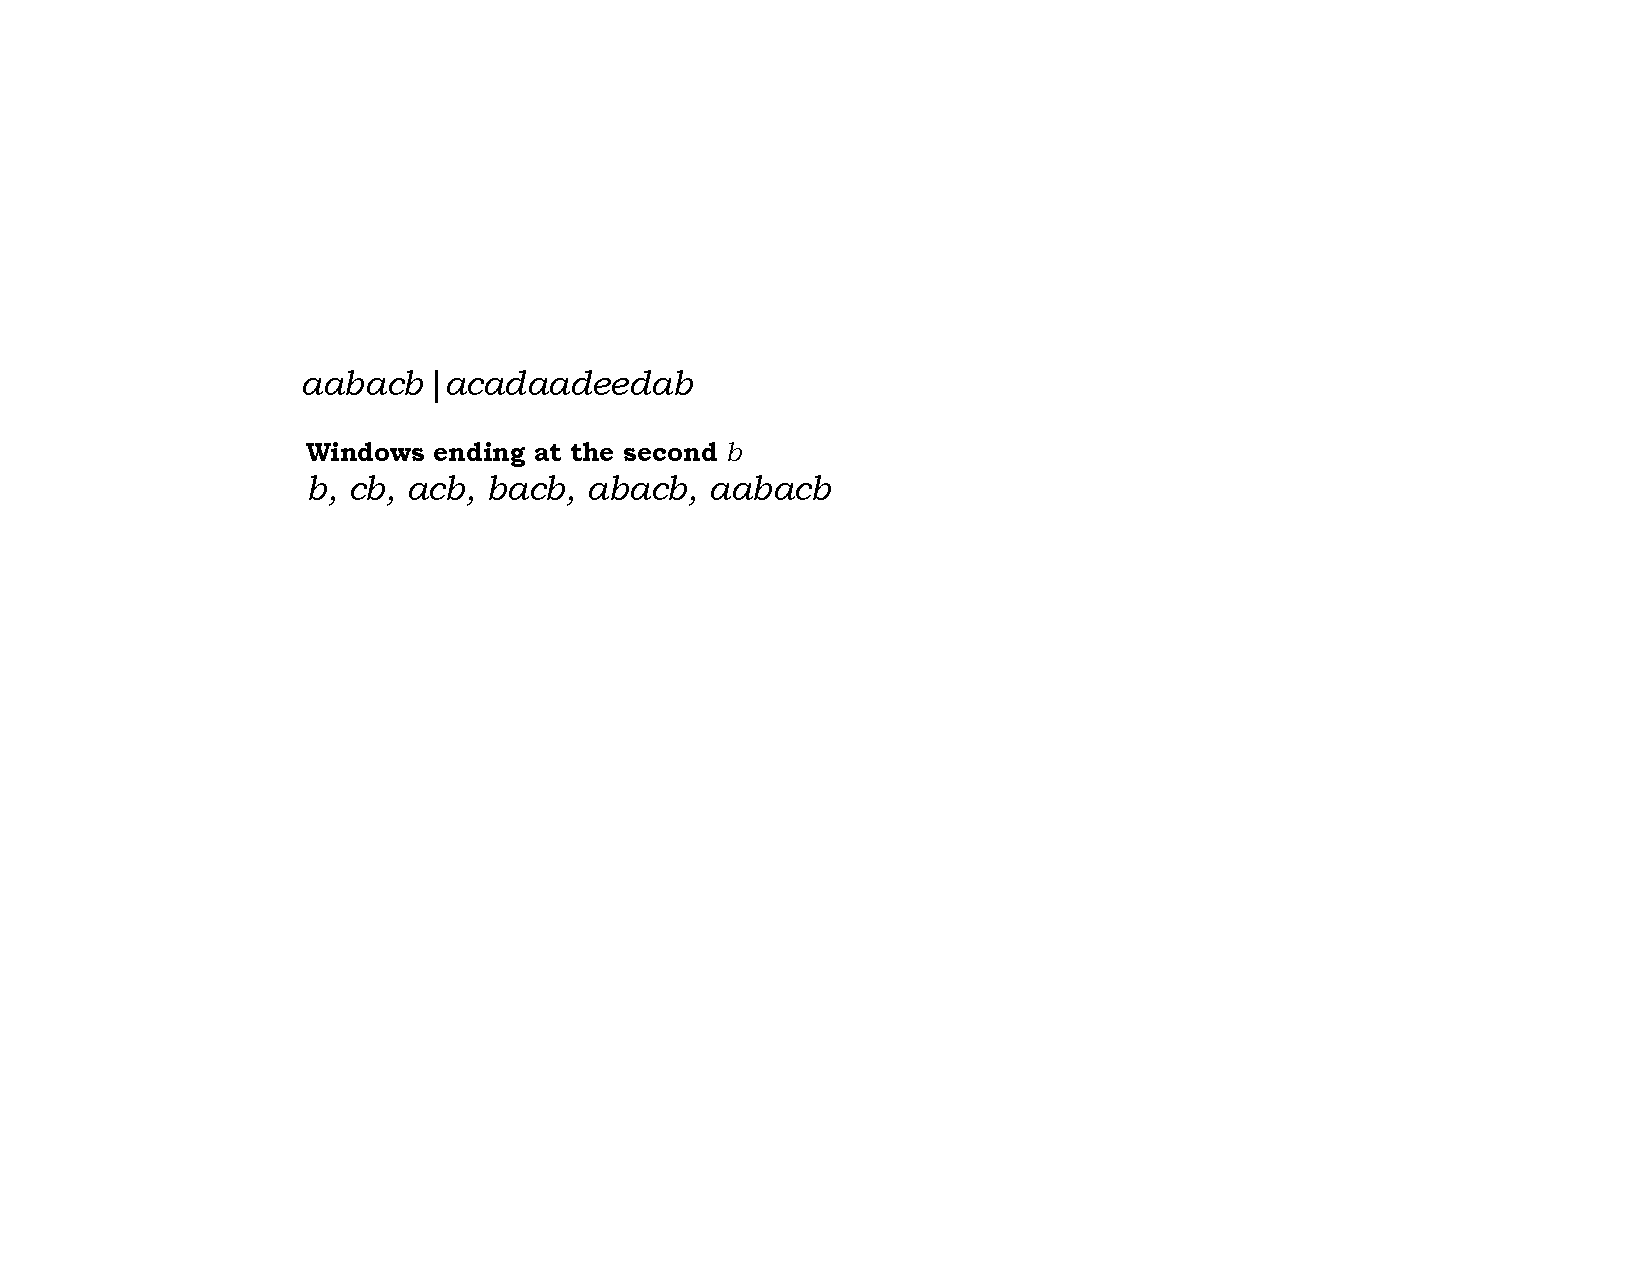
\includegraphics[width=0.7\textwidth]{figures/fp/pact09-illustration1}
  \caption{There are 3 different footprints for the 6 windows ending
    at the second $b$, so the 6 windows can be counted in 3 (instead of 6) steps.}
\label{fig:fp-illus1}
\end{figure}

\paragraph{Relative precision footprint size} By measuring data sizes
with a relative precision, for example, 99\% or 99.9\%, the number of
different footprint sizes becomes $O(\log m)$ instead of $m$ at each
step. Hence, the cost of the algorithm is reduced to $O(n\log m)$. This
approximation is acceptable because the use of large cache is affected
mostly by large footprints. For a large footprint, in most cases we
care about only the first few digits not the exact footprint.

The O(NlogM) algorithm improves the theorical time complexity of
footprint measurement. However, when we tried to apply it into
practical use, the profiling overhead turned out to be far more than
what we can afford in practice. It takes about 4 hours to get the
all-window footprint distribution for a 3 second run with O(NlogM)
algorithm. For a regular run of a typical SPEC2006 benchmarks which
takes about half an hour, the profiling run with O(NlogM) algorithm
will not have any results until three months later. We need techniques
that tell us results within hours or days, rather than months.

In this chapter, two techniques are proposed to efficiently measure
the program footprint. The first technique is called
\emph{all-footprint analysis}, because it measures the size of every
footprint. It can accomplish the measurement in $O(CKlogM)$ time,
where $CK$ is linear to the length of the trace and $M$ is the volume
of data accessed in the trace. The analysis is not fully accurate but
guarantees a constant precision, e.g. 99\%. The second technique is
called {\em average-footprint analysis}. For each window length, the
analysis shows the average size of footprints in all windows of this
length.  While the analysis gives the accurate average, it does not
measure the range or the distribution. We show that the average
footprint can be measured accurately in linear time $O(n)$ for a trace
of length $n$, regardless of the data size. Both techniques
significantly reduce measurement time of footprint. We apply shadow
sampling to average-footprint analysis to further reduce the time
overhead and make footprint an online measurable metric. We have
implemented both all-footprint analysis and average-footprint analysis
in Pin binary instrumentation tool and measured their performance with
SPEC2000 and SPEC2006 benchmark suites. The exciting results of speed
improvements are presented at the end of this Chapter.


\section{All-Footprint Analysis}
\label{sec:all-fp}

All-footprint analysis is a technique that applies trace compression
to O(NlogM) algorithm~\cite{DingC:PPOPP08}. It
takes the advantage of program locality to minimize computation steps,
reducing steps from O(N) to O(CK) where $C$ is a user specified
parameter and $K$ is a variable that highly depends on program locality and
$C$. The computational complexity of all-footprint analysis is
O(CKlogM), as introduced in detail in this section.

\subsection{Trace Compression: The CKM Algorithm}

Trace compression is proposed here to overcome the limitation of
existing techniques and further reduce the profiling overhead.
The basic idea is to analyze windows ending within a group of elements
in a cost similar to analyzing windows ending at a single element.
A user sets a threshold $c$.  The trace is divided into a
series of $k$ intervals called \emph{footprint intervals}.  Each
interval has $c$ distinct elements (except for the last interval,
which may have fewer than $c$ distinct elements). This is known as
trace compression.  It has been used by Kaplan et al. to shorten a
trace while still preserving the miss rate behavior~\cite{Kaplan+:TOMACS03}.
In footprint analysis, it allows us to traverse the trace interval by
interval rather than element by element.  The length of the trace is
reduced from $n$ to $k$. Next we describe the concepts and the
algorithm and show that this use of compression does not lose
precision in footprint analysis.

\begin{definition} {\em The footprint interval.}  Given a start point
  $x$ in a trace and a constant $c$, the footprint interval is the
  \emph{largest time window} from $x$ that contains accesses to
  exactly $c$ distinct data elements.
\end{definition}

Figure~\ref{fig:fp-illus2} (b) shows an example trace and its division into
footprint intervals.  The division is unique.  It maximizes the length
of each interval in order to minimize the number intervals.  We define
the length of an interval as the number of elements it has.  In this
example, the length is 9 for the first interval $I_1$ and 8 for the
second interval $I_2$.

We denote the series of footprint intervals by \emph{$I_i$},
data accesses by \emph{$\pi$}, the first access \emph{s} and the number
of footprint intervals \emph{K}. The trace partition is:

\[
I(\pi,s,c)=\cup_{i=1}^K I_i
\]

\noindent where $\forall i$, $I_i$ is a footprint interval
of size $c$; and $\forall i\ne j$, $I_i$ and $I_j$ do not overlap. 

Windows contained within a footprint interval have a footprint size
between 1 and $c$ and can be easily measured.  The more difficult
question is how to measure the footprint of a window that spans more
than one interval.  To show the algorithm, we first introduce some new
terms.  Assuming the current point is the start of the current
interval, we define

\begin{definition} {\sc Next-First-Accesses}, the first
  accesses to distinct data after the current point.
\label{cna}
\end{definition}

\begin{definition} {\sc Previous-Last-Accesses}, the last
  accesses to distinct data before the current point.
\label{cla}
\end{definition}

\begin{definition} {\sc Sub-intervals.} The current interval is divided
by the next-first-accesses into sub-intervals.
\end{definition}

\begin{definition} {\sc Past-Partitions.} The trace before the current
  point is divided by the previous-last-accesses into past partitions.
\end{definition}

\noindent Figure~\ref{fig:fp-illus2} shows for the first element in the
second interval, the 3 next-first-accesses, the 3
previous-last-accesses, the 3 sub-intervals, and the 3 past
partitions.  A past partition may span multiple intervals.

\begin{figure}[ht]
  \centering
  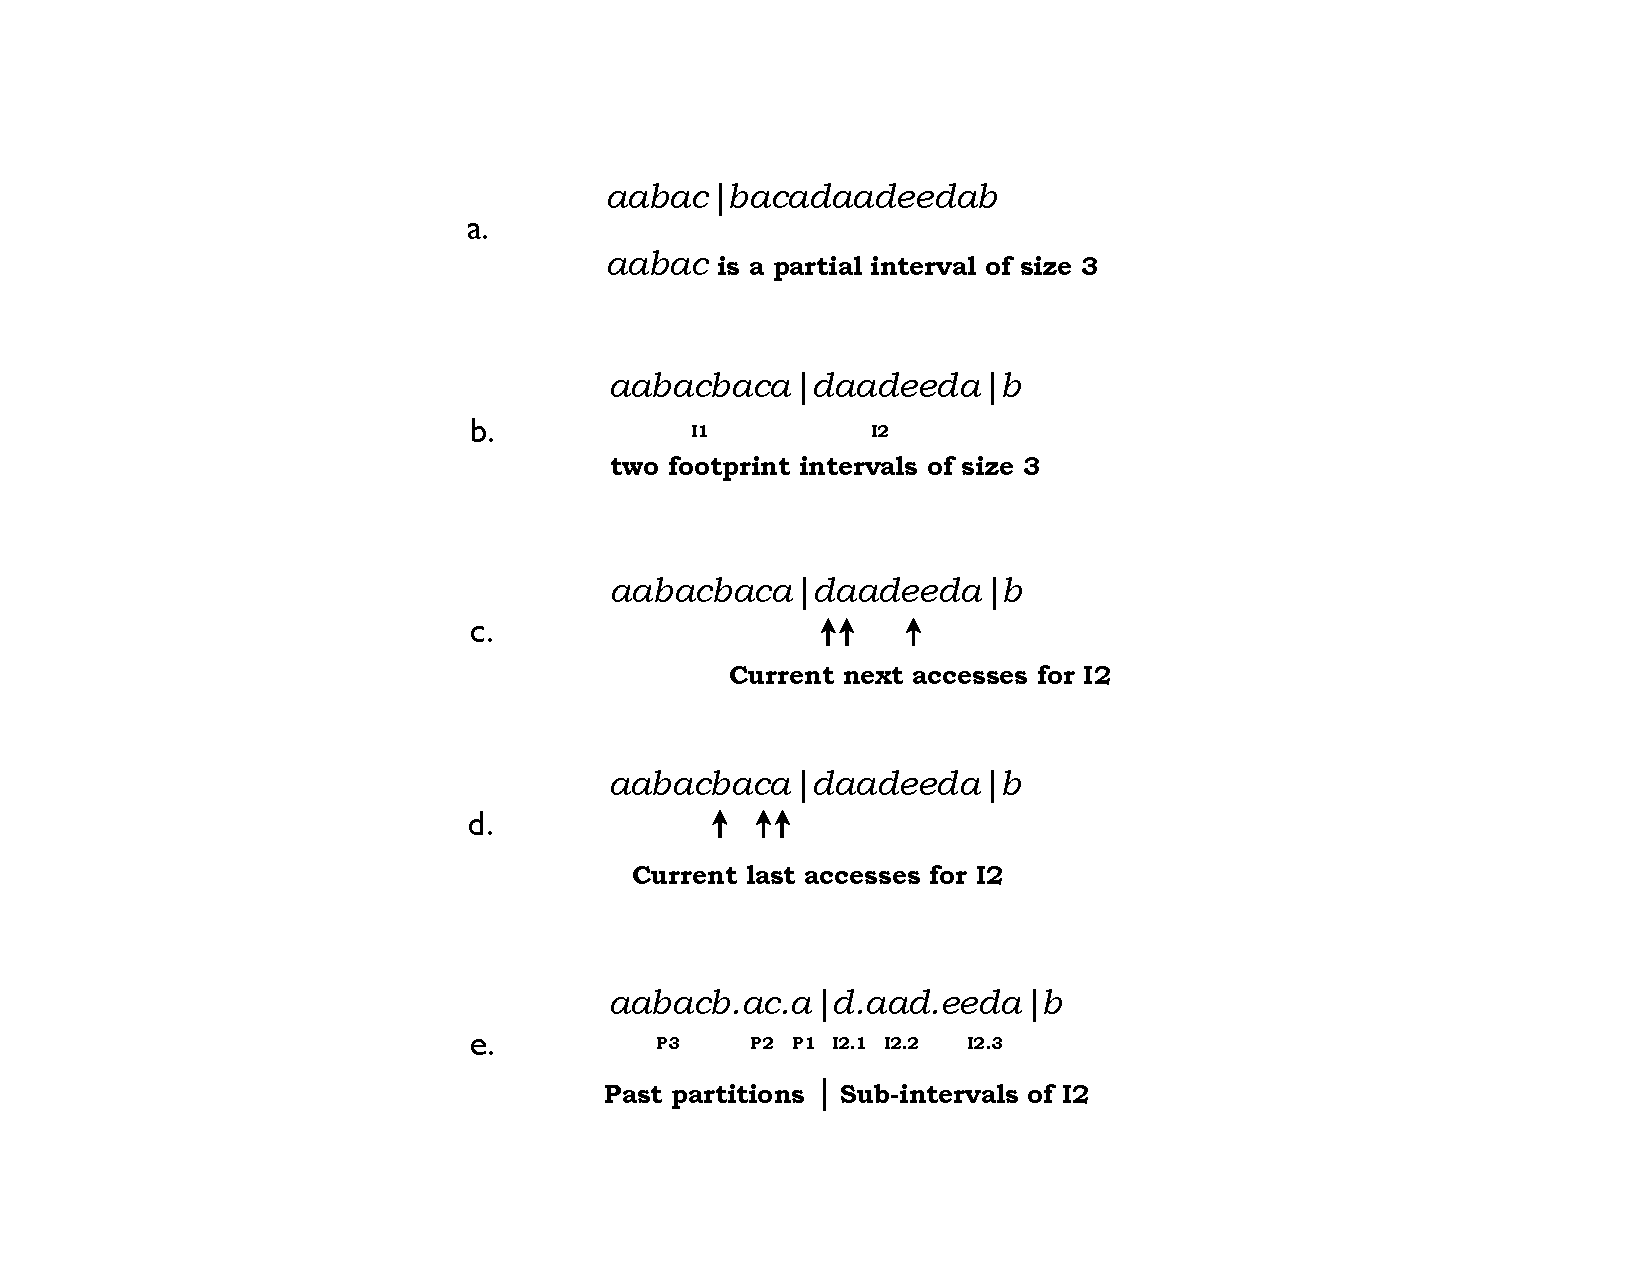
\includegraphics[width=0.7\textwidth]{figures/fp/pact09-illustration2}
\caption{Illustrations of the definitions used in the CKM algorithm}
\label{fig:fp-illus2}
\end{figure}

To count distinct footprint sizes in all windows, it is sufficient to count
between sub-interval and past partition markers, as is stated by the
following theorem.  Note that the footprint count for windows spanning
multiple intervals is precise regardless of the choice of $c$.

\begin{theorem} All windows starting within the same past-partition
  and ending within the same sub-interval have the same footprint.
\label{th1}
\end{theorem}

\begin{proof}
Suppose a time window starts from the past-partition $p$ and ends at
the sub-interval $s$. Suppose the successive data accesses within $p$
are $p_a,p_{a-1},...,p_1$ and the successive data accesses within $s$
are $s_1,s_2,...,s_b$. By definition, the previous-last-access in $p$
is $p_1$.  The next-first-access in $s$ is $s_1$.  Let $w^*$ be the
window from $p_1$ to $s_1$.  Let the footprint of $w^*$ be $fp^*$.

Fix the start position at $p_1$ and consider the window $w1$
that ends at $s_2$.  Since each sub-interval has only one
next-first-access, $s_2$ is not a first access and does not add to the
footprint.  The footprint of $w1$ is $fp^*$.  Similarly, we see that
all windows starting at $p_1$ and ending at $s_i, i=2,...,b$ have the
footprint $fp^*$.

Now let's fix the end position at $s_1$ and consider the window $w1$
that starts at $p_2$.  Since each past-partition has only one
previous-last-access, $p_2$ cannot be a previous-last-access and
therefore does not add to the size of the footprint.  The footprint of
$w1$ is $fp^*$.  Similarly, we see that all windows starting at
$p_a,...,p_2,p_1$ and ending at $s_1$ have the footprint $fp^*$.
Composing these two cases, we have the stated conclusion.  \qed

\end{proof}

By Theorem~\ref{th1}, the measurement of all-window footprints is
reduced to measuring the footprint in windows between every past
partition and every sub-interval.  The number of past-partitions is up
to $m$.  The number of sub-intervals is $c$.  Therefore, the number of
distinct footprints for windows ending at each footprint interval is
at most $cm$.  Since the number of the footprint intervals is $k$, the
time cost is then $O(ckm)$, hence the CKM algorithm.

We define the \emph{compression factor} as $\frac{n}{k}$, which is the
length of the trace over the number of intervals.  The compression
factor is minimal when $c=1$ and $k=n$ and maximal when $c=m$ and
$k=1$.  When $c$ increases from 1 to $m$, the compression factor
changes monotonically, as shown by the following lemma.

\begin{lemma} $k$ is a non-increasing function of $c$.
\end{lemma}

\begin{proof}
Suppose $e_i$ is the end position of footprint interval $I_i,
i=1,...,k$. We will prove by induction on $i$ that $e_i$ will never
move backward when $c$ is increased to $c*$.

In the base case, $I_1$ starts at the beginning of the trace, and
$e_1$ moves only forward in time when $c$ is increased.  Therefore,
the start position of $I_2$ does not move backwards.

Suppose start position of $I_i, i\geq 2$ does not move backwards,
and the next interval starting with the new start position and ending
with previous $e_i$ has a footprint of no more than $c$. As a
result, the new $e_i$ will only move forward in time when $c$ is
increased to $c^*$. \qed
\end{proof}

\begin{comment}
Figure~\ref{code:CKM} shows the design of the CKM algorithm.  Three
global variables are used to maintain interval states--the start time
of the current interval, the current size of interval, and the start
time of current sub-interval.  They are initialized to 1, $c$ and 0
correspondingly.

\newlength{\movinc}
\setlength{\movinc}{0.3cm}
\newcommand{\move}[1]{\hspace{#1\movinc}}
\begin{figure}[h!]
  \subfigure{
    \begin{minipage}[b]{0.4\textwidth}
      % \centering
      \begingroup \tt \footnotesize
      \begin{tabular}{l}
        {\bf data declarations}\\
        \move{1}cur\_interval\_size = C\\
        \move{1}cur\_interval\_start = 1\\
        \move{1}cur\_sub\_start = 0\\
        \move{1}//current sub-interval start time\\
        \vspace{0.2cm}\\
        {\bf algorithm} Footprint(last, current)\\
        \move{1}//inputs are last and current access time\\
        \move{1}if (last<cur\_interval\_start)\\
        \move{2}//new data access for current interval\\
        \move{2}//that is, current sub-interval ends\\
        \move{2}CalcSubinterval(cur\_sub\_start,\\ 
        \move{3}current-1, cur\_interval\_size)\\
        \move{2}cur\_sub\_start = current\\
        \move{2}if (last==0)\\
        \move{3}M++\\
        \move{2}endif\\
        \move{2}if (current\_interval\_size != C)\\
        \move{3}current\_interval\_size++\\
        \move{2}else//current interval ends\\
        \move{3}K++\\
        \move{3}UpdatePastPartitions()\\ 
        \move{3}cur\_interval\_size = 1\\
        \move{2}endif\\
        \move{3}TraceSearchDelete(last)\\
        \move{1}endif\\
        {\bf end algorithm}\\
      \end{tabular}
      \endgroup
    \end{minipage}
    \label{part1}
  }\hfill
  \subfigure{
    \begin{minipage}[b]{0.4\textwidth}
      % \centering
      \begingroup \tt \footnotesize
      \begin{tabular}{l}
        {\bf subroutine} \\
        CalcSubinterval(start, end, base\_fp)\\
        \move{1}fp = base\_fp\\ 
        \move{1}foreach p in past partition \\
        \move{2}//ordered from most recent\\ 
        \move{2}//to least recent\\
        \move{2}fp += size(p)\\
        \move{2}foreach w in windows starting in \\
        \move{2}current past partition and ending \\
        \move{2}in current subinterval\\
        \move{3}ws = length(w)\\
        \move{3}//Footprints and windows are organized\\
        \move{3}//in bins according to their size.\\ 
        \move{3}//bin\_idx function is used to\\ 
        \move{3}//return the index of bin corresponding\\
        \move{3}//to the input.\\
        \move{3}data[bin\_idx(ws)][bin\_idx(fp)]++\\
        \move{2}end foreach w\\
        \move{1}end foreach p\\
        {\bf end subroutine}\\
        \vspace{0.2cm}\\
        {\bf subroutine} UpdatePastPartitions\\
        \move{1}new\_list <- past-partitions \\
        \move{4}within current region\\
        \move{1}append new\_list to existing \\
        \move{4}past-partitions list\\
        {\bf end subroutine}
        % \vspace{0.2cm}\\
      \end{tabular}
      \endgroup
    \end{minipage}
  }\\
  \caption{CKM Algorithm for All-Footprint Analysis}
  \label{code:CKM}
\end{figure}


For each data access, we record the current time as its access time
and find its last access time (most recently accessed time) using a
hash-table. The cost of finding the last access time is not considered
in our discussion. The main algorithm is called to check whether any
calculations of footprints are need here. If the last access time of
current data access is bigger than the start time of current
footprint-interval, then the current data access must have been accessed
somewhere within the current footprint-interval before the current time stamp,
which means, the current data access is not a current-next-access for
the current interval by definition~\ref{cna}. We do not have to
care about this access and can just move to the next data
access. Otherwise if last access time of current data access is
smaller than the current region start time, then current data access
is new to current footprint interval, which means, current data access
is a current-next-access for current interval. Since sub-intervals are
divided by current-next-accesses, the arrival of new
current-next-access implies the ending of current sub-interval. With
the start time and end time of current sub-interval, we can calculate
the footprints of windows which are ending at current
sub-interval. After the calculation, a new sub-interval is started.

Notice that if a data access is new to the current interval, it may
also be the first access in the trace. If the last access time is 0,
we should increase the total data size correspondingly. If current
interval size is less than the upper bound $c$ (the capacity of each
footprint interval defined by the algorithm), we simply add current
access into current interval and increase the interval
size. Otherwise, if current interval size is no smaller than $c$, then
current data access cannot be added to current interval any more,
which means, current data access starts a new interval. In this case,
we should update the number of existing intervals, convert current
interval into past-partitions, and build a new current interval.
\end{comment}


\subsection{Further improvement: The CKlogM Algorithm}

We combine the relative precision NlogM algorithm and the trace
compression CKM algorithm as follows.  Instead of using
previous-last-accesses in the CKM algorithm, we use the the relative
precision footprint sizes described in ~\cite{DingC:PPOPP08}.
The approximation divides the past
trace into $O(\log m)$ past partitions.  The number of
next-first-accesses is still $c$, and the number of intervals is $k$.
The total cost becomes $O(ck\log m)$, hence the CKlogM algorithm.

\paragraph{CKlogM algorithm compared with NlogM algorithm} In extreme
case, CK could be as large as N. While CKlogM does not improve the
theoretical time complexity of NlogM algorithm, it has great gain in
practice because of program locality. With $C$ carefully chosen, the
CKlogM algorithm improves the measurement by a factor of 100 or
more. We will include a more detailed discussion in
Section~\ref{subsec:fp-eval-all-fp} with supporting experimental results.

\section{Average Footprint Analysis}
\label{sec:avg-fp}

With all-footprint analysis, we get most detailed information of all window
footprint distribution. With full distribution serving as the
reference, we are now able to try different approximation approaches
and evaluate their accuracy. Average statistics turns out to be a good
approximation that is presentative and easy to
measure. In this section, we first define average footprint and
then introduce a linear time algorithm that measures the average
statistics without losing any precision.

\subsection{Definitions}

Let $W$ be the set of ${{n}\choose{2}}$ windows of a length-$n$ trace.
Each window $w = <t, v>$ has a length $t$ and a footprint $v$.  Let
$I(p)$ be a boolean function returning 1 when $p$ is true and 0
otherwise.  The footprint function $\overline{fp}(t)$ averages over
all windows of length $t$:

$$\overline{fp}(t) = \frac{\sum_{w_i \in W} v_i I( t_i = t
  )}{\sum_{w_i \in W} I(t_i = t)} = \frac{\sum_{w_i \in W} v_i I( t_i = t
  )}{ n - t + 1} $$


For example, the trace ``abbb'' has 3 windows of length 2: ``ab'',
``bb'', and ``bb''.  The corresponding footprints are 2, 1, and 1, so
$\overline{fp}(2) = (2+1+1)/3 = 4/3$.  

\subsection{O(n) Algorithm}

There is a linear-time algorithm that calculates the precise average
footprint for all execution windows of a trace.  Let $n,m$ be the
length of the trace and the number of distinct data used in the trace.  The
algorithm first measures the follow three quantities: 

\begin{itemize}
  \item the distribution of the time distances of all data reuses ($n-m$ distances)
  \item the first-access times of all distinct data ($m$
  access times)
\item the last-access times of all distinct data (exact definition
  later, $m$
  access times)
\end{itemize}

The three quantities can be measured by a single pass over the
trace using a hash table with one entry for each distinct
data.  The cost is linear, $O(n)$ in time and $O(m)$ in space.

The three measures are the inputs to a formula $\overline{fp}(w)$.
For any window size $w (0< w \le N)$, $\overline{fp}(w)$ computes the average
footprint for all windows of size $w$.  In other words, the formula computes
the average footprint for windows of all sizes without having to
inspect the trace
again.  In the rest of the section, we derive the formula and discuss
its complexity.

The main idea of the formula is \emph{differential counting}, which
counts the difference in the footprint between consecutive windows.  For
any window size $w$, we start with the footprint in the first window
and then compute its increase or decrease as the window moves forward
in the trace.  The first-access times are sufficient to compute the
footprint of the first window.  The change in later windows depends on two metrics on
each trace element $d_i$: the forward time distance $fwd(d_i)$
and the backward time distance $bwd(d_i)$.  Let datum $x$ be accessed
at $d_i$.  Let the closest accesses of $x$ be
$d_j$ before $d_i$ and $d_k$ after $d_i$.  Then $fwd(d_i) = k - i$ and
$bwd(d_i) = i - j$.

% fwd and bwd are labels on automatic shifts in cars: forward and
% backward.  Here the middle w also reminds a reader that we are
% talking about a window of size w.

The forward and backward time distances determine the change 
of footprint between consecutive windows.  The relation is shown
in Figure~\ref{fig:illus-aver-fp}.  

\begin{figure}[h!]
\centering
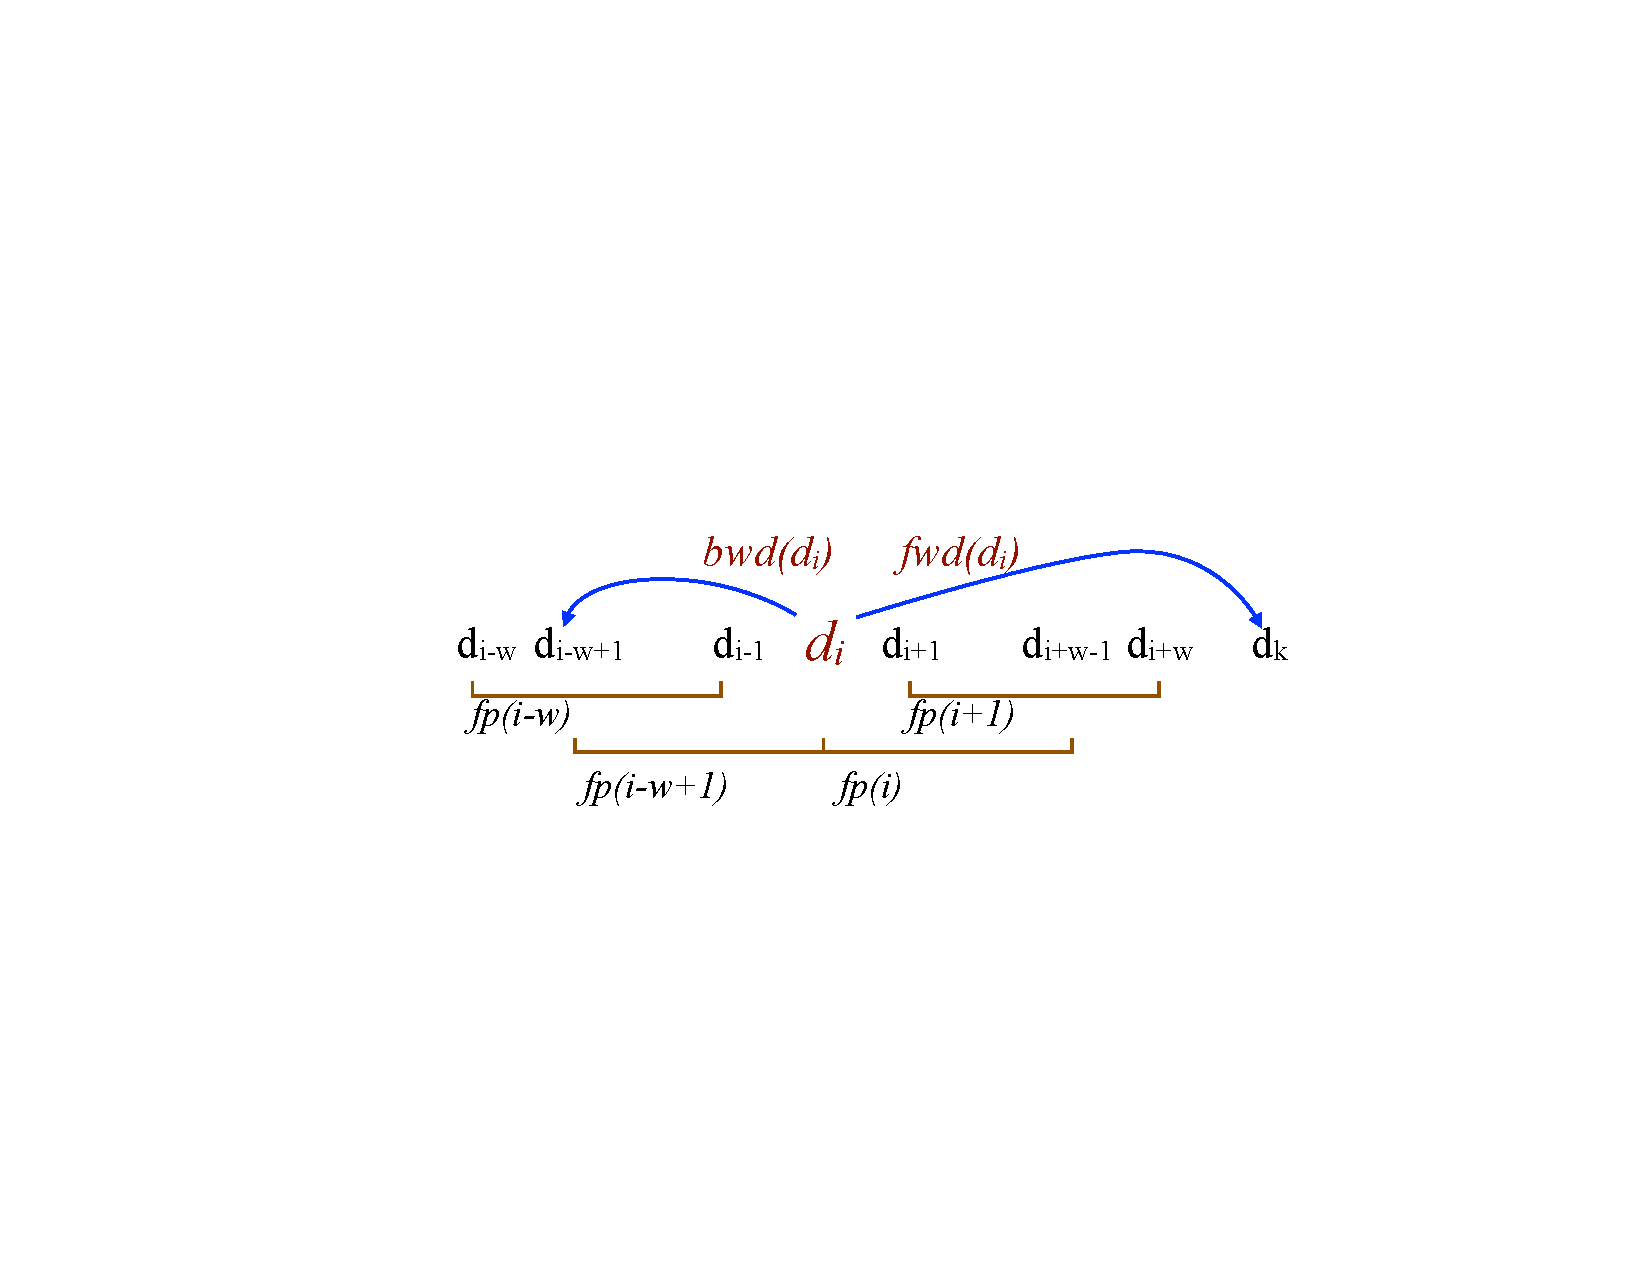
\includegraphics[width=7.8cm]{figures/fp/di_fig}
\caption{An illustration how the forward and backward (reuse) time
  distance influences the change in footprint between consecutive
  windows}
\label{fig:illus-aver-fp}
\end{figure}

Let the footprint of a $w$-size window starting at $i$ be $fp(i)$.
Each element $d_i$ in the trace affects the footprint of $w$ windows:
$fp(i-w+1), fp(i-w+2), \dots, fp(i)$.  In differential counting, we
consider only the effect of $d_i$ on two pairs of windows: the change
from $fp(i-w)$ to $fp(i-w+1)$ when $d_i$ enters into its first window
and the change from $fp(i)$ to $fp(i+1)$ when $d_i$ exits from its
last window of influence.   Figure~\ref{fig:illus-aver-fp} shows $d_i$ and 
the two pairs of windows where $d_i$ enters between the first pair and
exits between the second pair.

When $d_i$ enters, it does not increase the footprint $fp(i-w)$ if the
same datum was previously accessed within $fp(i-w+1)$, which means
that its backward time distance is no greater than $w$ ($bwd(d_i) \le
w$).  This is the case illustrated in Figure~\ref{fig:illus-aver-fp}.  Otherwise,
$d_i$ adds 1 to the footprint $fp(i-w)$.  Similarly, when $d_i$ exits
from $fp(i)$, the departure does not change $fp(i+1)$ if $fwd(d_i) \le
w$; otherwise, it subtracts 1 from $fp(i+1)$, as the case
illustrated in Figure~\ref{fig:illus-aver-fp}.

The footprint $fp(i+1)$ depends on three factors: the footprint
$fp(i)$, the contribution of the entering $d_{i+w}$,
and the detraction of the exiting $d_i$.  The footprint of all windows
is then computed by adding these differences.  Next we formulate
this computation.  We use the following notations.

\begin{itemize}
\item $n, m, w$: the length of the trace, the size of data, and the
  window size of interest
\item $d_i$:  the $i$-th trace access
\item $fp(i)$: the footprint of the window from $d_i$ to $d_{i+w-1}$
  (including $d_i$ and $d_{i+w-1}$)
\item $bwd(d_i)$: the backward reuse time distance of $d_i$, $\infty$ if
  $d_i$ is the first access.
\item $fwd(d_i)$: the forward reuse time distance of $d_i$, $\infty$ if
  $d_i$ is the last access.
\item $I(p)$: a boolean function that returns 1 if $p$ is true and 0
  otherwise.  For example, $I(bwd(d_i)>w)$ gives the contribution by
  $d_i$, which is 1 if $bwd(d)>w$ and 0 otherwise.  Similarly,
  $I(fwd(d_i)>w)$ gives the detraction of $d_i$, 1 if $fwd(d)>w$ and 0
  otherwise.
\end{itemize}

The total size of the footprints in all windows of length $w$, when divided by the
number of windows $n-w+1$, is the average footprint, as shown next
in Equation~\ref{eq2}.

\begin{equation}
\label{eq2}
\small
\overline{fp}(w)= \frac{1}{n-w+1}\sum_{i=1}^{n-w+1}fp(i)
\end{equation}

\noindent Since 

\begin{equation}
\label{eq3}
fp(i+1) = fp(i)+I(bwd(d_{i+w})>w)-I(fwd(d_i)>w)
\end{equation}

\noindent Expanding Equation~\ref{eq2} using Equation~\ref{eq3},
we have three components in the average footprint:

\begin{eqnarray}
\label{eq4}
\small
&\overline{fp}(w) = & fp(1) + \frac{1}{n-w+1} (\sum_{i=w+1}^{n}(n-i+1)I(bwd(d_i)>w)  \nonumber \\
& & - \sum_{i=1}^{n-w}(n-i+1-w)I(fwd(d_i)>w) )
\end{eqnarray}

Next we compute each component separately. The footprint of the first
window of length $w$ is 
 
\begin{equation}
\label{eq5}
fp(1)=\sum_{i=1}^{w}I(bwd(d_i)=\infty)
\end{equation}

In the next component, we split the forward time distances into two
groups: finite and infinite distances.  The summation order of the 
finite distances can be changed from 1 to $n$ instead of from $w+1$ to
$n$.

\begin{eqnarray}
\label{eq6}
&\ &\sum_{i=w+1}^{n}(n-i+1)I(bwd(d_i)>w) \\
&=& \sum_{i=w+1}^{n}(n-i+1)I(w<bwd(d_i)<\infty)+\sum_{i=w+1}^{n}(n-i+1)I(bwd(d_i)=\infty)\nonumber\\
&=&
\sum_{i=1}^{n}(n-i+1)I(w<bwd(d_i)<\infty)+\sum_{i=w+1}^{n}(n-i+1)I(bwd(d_i)=\infty)\nonumber
\end{eqnarray}


\noindent Similarly, we decompose and simplify the forward distances:

\begin{eqnarray}
\label{eq7}
&\ &\sum_{i=1}^{n-w}(n-i+1-w)I(fwd(d_i)>w) \\
&=& \sum_{i=1}^{n}(n-i+1-w)I(w<fwd(d_i)<\infty)+\sum_{i=1}^{n-w}(n-i+1-w)I(fwd(d_i)=\infty)\nonumber
\end{eqnarray}

Since forward reuse distance and backward reuse distance is a
one-to-one mapping, that is, for any reuse pair $d_i$ and $d_j$,
$fwd(d_i)=bwd(d_j)$. Denote the reuse distance between $d_i$ and
$d_j$ by $t$($t=j-i$), we have the following equation.

\begin{eqnarray}
\label{eq8}
&\ &(n-j+1)I(w<bwd(d_j)<\infty)-(n-i+1-w)I(w<fwd(d_i)<\infty)\nonumber\\
&=&(w-t)I(w<t<\infty)
\end{eqnarray}

Combining the Equations~\ref{eq5}, \ref{eq6}, \ref{eq7}, and \ref{eq8}, we can now
expand Equation~\ref{eq4}.  Instead of using individual accesses,
we now use the three inputs, 
defined as follows:

\begin{itemize}
\item $f_i$: the first access time of the $i$-th datum
\item $l_i$: the \emph{reverse} last access time of the $i$-th datum.
  If the last access is at position $x$, $l_i = n+1-x$, that is, the
  first access time in the reverse trace.
\item $r_t$: the number of accesses with a reuse time distance $t$
\end{itemize}

\begin{eqnarray}
\small
\label{aver-fp-eq}
&\overline{fp}(w)&=m+\frac{1}{n-w+1}\\
&\ &( \sum_{i=1}^{m}(w-f_i)I(f_i>w)+\sum_{i=1}^{m}(w-l_i)I(l_i>w)\nonumber+\sum_{t=1}^{n-1}(w-t)I(t>w) r_t )\nonumber
\end{eqnarray}

The formula of Equation~\ref{aver-fp-eq} passes the sanity check that the
average footprint $\overline{fp}(w)$ is at most the data size $m$, and
the footprint of the whole trace ($w=n$) is $m$.  Fixing the window
length $w$ and ignoring the effect of first and last accesses, we see
that the footprint decreases if more reuse time distances
($r_t$) have larger values ($t$).  This suggests that improving
locality reduces the average footprint.  For example, if we double the
length of a trace by repeating each element twice, the length of the
long time distances would double, and the average footprint would
drop.

For each window length $w$, the Equation~\ref{aver-fp-eq} can be computed in
time $O(w)$.  If we limit to consider only window sizes of a
logarithmic scale, the formula can be represented and evaluated in
$O(\log w)$ time.

\subsection{Monotonicity}
\label{subsec:aver-fp-mono}
\newcommand{\qedblob}{\mbox{\rule[-1.5pt]{5pt}{10.5pt}}}
\def\qed{{\ \nolinebreak\hfill\mbox{\qedblob\quad}}}

\begin{theorem} The average footprint $\overline{fp}(w)$ is non-decreasing.
\label{th1}
\end{theorem}

\begin{proof}
  Let $w_i^k$ denotes the $i$-th window whose size is $k$, $f(w_i^k)$
  denotes the footprint of the $i$-th window whose size is $k$.  We
  prove that, $\forall k$, $0<k \le n$, $\overline{fp}(k+1) \ge
  \overline{fp}(k)$.

First, $\forall i$, $0<i \le n-k$, the following holds because
$w_i^{k}$ and $w_{i+1}^{k}$ are both contained in $w_i^{k+1}$:

\begin{itemize}
\item $f(w_i^{k+1}) \ge f(w_i^{k})$ 
\item $f(w_i^{k+1}) \ge f(w_{i+1}^{k})$ 
\end{itemize}

\noindent In addition, we have $\forall k$,  $0<k\le n, \exists j$, $0<j \le
n-k+1$, such that, $f(w_j^k) \le \overline{fp}(k)$.  Now then
\begin{eqnarray}
\label{eq9}
\overline{fp}(k+1) &=&\frac{1}{n-k}\sum_{i=1}^{n-k}f(w_i^{k+1}) \nonumber \\
&=&\frac{1}{n-k}[\sum_{i=1}^{j-1}f(w_i^{k+1})+\sum_{i=j}^{n-k}f(w_i^{k+1})] \nonumber \\
&\ge&\frac{1}{n-k}[\sum_{i=1}^{j-1}f(w_i^{k})+\sum_{i=j}^{n-k}f(w_{i+1}^{k})] \nonumber \\
&=&\frac{1}{n-k}[\sum_{i=1}^{j-1}f(w_i^{k})+\sum_{i=j+1}^{n-k+1}f(w_{i}^{k})] \nonumber \\
&=&\frac{1}{n-k}[\sum_{i=1}^{n-k+1}f(w_i^{k})-f(w_j^k)] \nonumber \\
&=&\frac{1}{n-k}[(n-k+1)\overline{fp}(k)-f(w_j^k)] \nonumber \\
&=&\overline{fp}(k)+\frac{1}{n-k}[\overline{fp}(k)-f(w_j^k)] \nonumber \\
&\ge&\overline{fp}(k) \nonumber
\end{eqnarray}
%\qed
\end{proof}


\subsection{Complexity Discussion}

To compute average footprint curve, we need the compute footprint for
all window lengths. With Equation~\ref{aver-fp-eq}, we are able to
compute average footprint for each window in time $O(w)$, where $w$
ranges from 1 to $n$. An simple calculation will say the full curve
needs a total computing time of $O(n^2)$. However, with carefully
reusing the intermediate results, we care able to compute the whole
curve in O(n) with the following steps. We combine reuse distance(t), first
access distance(f), and last access distance(l), and use two arrays
$count$ and $count_i$ to record the statistic information. Both
$count$ and $count_i$ are of size $n$. $count[i]$ contains the count
of how many reuse distance(t), first access distance(f), and last
access distance(l) equal to $i$, while $count_i[i]$ equals to
$i*count[i]$. Equation~\ref{aver-fp-eq} can be further simplied as
below. 

\begin{eqnarray}
%\label{aver-fp-eq}
&\overline{fp}(w) & =  m - \frac{1}{n-w+1} (
  \sum_{i=w}^{n}(count_i[i]-w*count[i]))\nonumber\\
&\ &=\frac{1}{n-w+1}(m*(n-w+1)-\sum_{i=1}^{n}(count_i[i]-w*count[i]) +\nonumber\\
&\ &\sum_{i=1}^{w-1}(count_i[i]-w*count[i]))\nonumber\\
&\ &=\frac{1}{n-w+1}(m*(n-w+1)-\sum_{i=1}^{n}count_i[i]+w\sum_{i=1}^{n}count[i] +\nonumber\\
&\ &\sum_{i=1}^{w-1}count_i[i]-w\sum_{i=1}^{w-1}count[i])\nonumber\\
&\ &=\frac{1}{n-w+1}(m*(n-w+1)-m(n+1)+w(n+m)+\nonumber\\
&\ &\sum_{i=1}^{w-1}count_i[i]-w\sum_{i=1}^{w-1}count[i])\nonumber\\
&\ &=\frac{1}{n-w+1}((n-count[i])*w + count_i[i])
\end{eqnarray}

The simplied equation can be easily calculated with
the procedure shown in Figure~\ref{alg:aver-fp} within time of O(n).

\renewcommand{\algorithmicrequire}{\textbf{Procedure}}
\begin{figure}[h!]
  \centering
  \begin{minipage}{\linewidth}
    \begin{algorithmic}[1]
      \REQUIRE array $count[n]$, $count_i[n]$, where $count[i]$ contains the
      count of how many reuse distance(r)/first access
      distance(f)/last access distance(l) equal to $i$, $count_i[i]$ contains $i*count[i]$.
      \STATE return fp[n], where fp[i] is the average footprint of
      windows of length $i$.
      \STATE $sum$ = 0, $sum_i$ = 0;
      \FOR{ w = 1 \TO n }
      \STATE  fp[w] = ((n - $sum$) * w + $sum_i$) / (n - w + 1)
      \STATE  $sum$ += $count$[w]
      \STATE  $sum_i$ += $count_i$[w]
      \ENDFOR
    \end{algorithmic}
    \caption{Calculation of average footprint curve}
    \label{alg:aver-fp}
  \end{minipage}
\end{figure}

\section{Footprint Sampling}
\label{sec:sampling}
Sampling is widely used to reduce measurement overhead. We apply
sampling to average footprint by first measuring average footprint for
sampled traces and then take the average over all the
segments. Sampling happened every $t$ seconds, and lasted until
the trace contains at least $c$ distinct data. Parameter $t$ and $c$
changes according to the context. For example, when we concern about
 footprint less than cache size, we use cache size as the $c$
 value. The sampling with $c$ equals cache size is called
 \emph{lifetime sampling}. More discussion on lifetime sampling will
 show in Section~\ref{sec:lf-sampling}. We applied sampling to speedup average
 footprint measurement as below. When a program
starts, we set the system timer to interrupt every $t$ seconds.
The interrupt handler is shown in Figure~\ref{alg:fp-sampling}.  It forks
a sampling task and attaches the binary rewriting tool
Pin~\cite{Pin:PLDI05}.  The Pin tool instruments the sampling process
to collect its data access trace, measures all-window footprint using
average-footprint analysis described in Section~\ref{sec:avg-fp}.

\renewcommand{\algorithmicrequire}{\textbf{Procedure}}

\begin{figure}[t!]
 \centering
 \begin{minipage}{\linewidth}
   \begin{algorithmic}[1]
     \REQUIRE timer interrupt handler, called whenever a program receives the
     timer interrupt
     \STATE Return if the sampling flag is up
     \STATE Set the sampling flag
     \STATE $pid \gets fork()$
     \IF{$pid = 0$}
        \STATE Turn off the timer
         \STATE Attach the Pin tool and begin sampling until seeing
         $c$ distinct memory accesses
         \STATE Exit
     \ELSE
         \STATE Reset the timer to interrupt in $t$ seconds
         \STATE Wait for $pid$ to finish
         \STATE Clear the sampling flag
         \STATE Return
     \ENDIF
   \end{algorithmic}
   \caption{The timer-interrupt handler for locality sampling}
   \label{alg:fp-sampling}
 \end{minipage}
\end{figure}



\section{Evaluation}

\subsection{Experiment Setup}
\label{subsec:fp-eval-setup}
To precisely quantify the efficiency of different techniques, we did
three sets of comparisons, different set on potentially different
benchmark sets, as listed below. Since profiling is
machine-independent, we use a Linux cluster for profiling different
benchmarks in parallel to save time.  Each node has two 3.2GHz 64-bit
Intel Xeon processors with 1MB L2 cache each and 6GB physical memory total.

\begin{itemize}
\item All-footprint analysis efficiency, which compares the speed of
  all-footprint analysis(CKlogM algorithm) with the previously fastest
  O(NlogM) algorithm.
\item Average-footprint analysis efficiency, which compare the speed
  of average-footprint analysis with all-footprint analysis. 
\item Efficiency of footprint sampling, which compare the sampling
  analysis speed with both original runtime(without any
  instrumentation) and average-footprint analysis.
\end{itemize}

Depends on the comparison reference, the comparison are conducted on
different benchmark sets and with different instrumentation tools. For
example, Pin-based instrumentation tool collects the trace about 10
times as long as what GCC-based tool collects for the same program
because Pin includes the library traces in; since O(NlogM) analysis
is very slow even for short traces, we don't implement it with Pin, but
with GCC instead. We conduct NlogM vs. CKlogM comparison only on
SPEC2000 benchmarks but not on SPEC2006 also because of the slow speed
of NlogM analysis.

\subsection{Efficiency of All-Footprint Analysis}
\label{subsec:fp-eval-all-fp}

We implemented both our all-footprint
  O(CKlogM) analysis and the previously fastest O(NlogM) analysis in a
  modified GCC 4.1 compiler with ``-O3'' flag. The compiler is
  modified to instrument each memory access and generate the data
  access trace when the program runs. The O(NlogM) analysis is too slow that it
  finished only 12 benchmarks of 26 SPEC2000 test suite. We will only
  compare the performance on these 12 benchmarks. The precision of
  both analysis is set to 90\%. 

\paragraph{Footprint distribution overview} Figure~\ref{fig:all-fp-group} shows the full distribution of
all-window footprint in 4 of the 12 benchmarks.  While
every program has a different looking footprint, we choose these 4
because they demonstrate the range of variations.  Each graph shows
window size, measured in number of data accesses with exponential scale,
in the $x$-axis and footprint, measured in bytes, in the $y$-axis.
It's worth to note, since our measurements are based on 64-byte blocks 
the footprint sizes are always multiples of 64.   At each window size,
each graph shows five footprint numbers: the minimal size {\tt min}, the
maximal size {\tt max}, the {\tt median}, and the two footprints whose
size is higher than {\tt 90\%} and {\tt 10\%} of footprints.  We
connect the points into a line, so each distribution is drawn with
five curves.  In probability terms, a point $(x, y)$ on the n\% curve
indicates that a window of $x$ data accesses has n\% chance to have a
footprint smaller than $y$.

\newlength{\figwid}
\setlength{\figwid}{0.46\textwidth}

\begin{figure}[!h]
  \subfigure[{\bf Gzip} has constant-size median working sets for
  windows from 1 million to 256 million accesses.]  {
    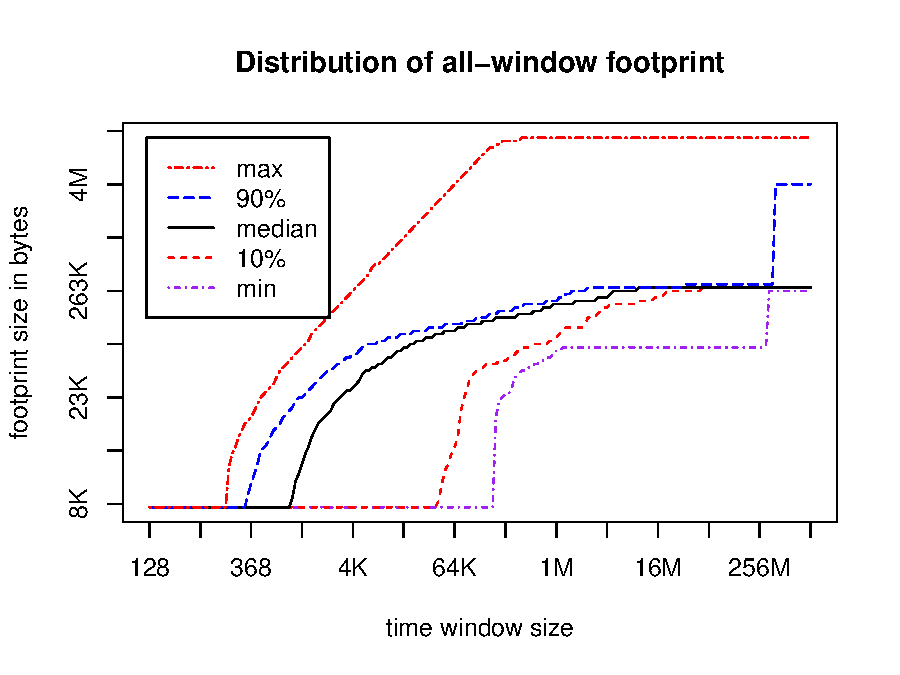
\includegraphics[width=\figwid]{figures/fp/164_gzip_ref}
    \label{fp-gzip-128}
  }\hfill \subfigure[{\bf Bzip2} has a larger working set than
  \emph{Gzip} for windows larger than 256 thousand accesses.] {
    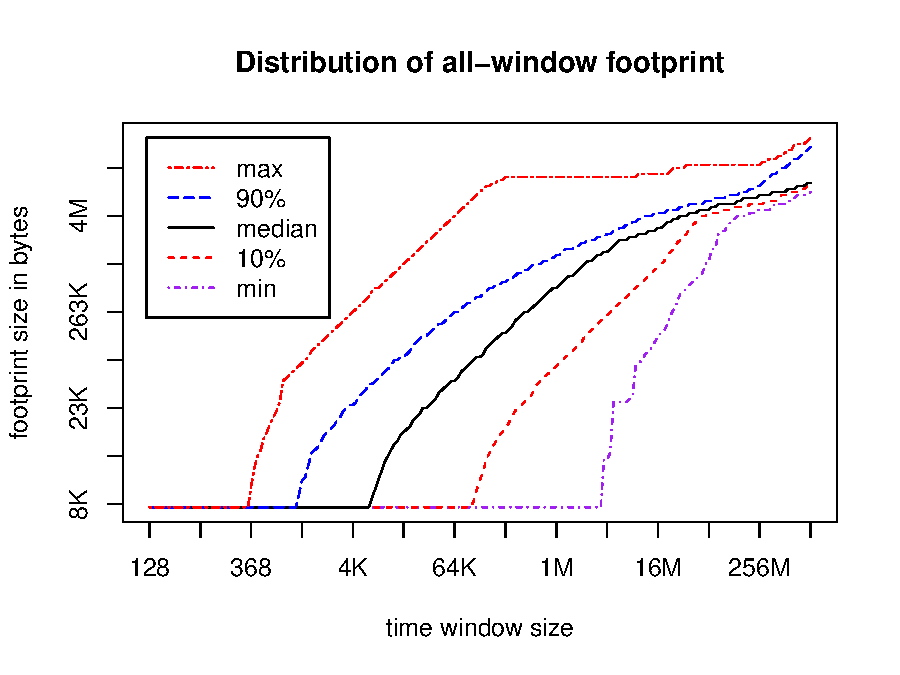
\includegraphics[width=\figwid]{figures/fp/256_bzip2_ref}
    \label{fp-bzip2-128}
  }\hfill
  \subfigure[{\bf Equake} has a streaming access pattern.  The
  footprint increases linearly with the window size.]{
    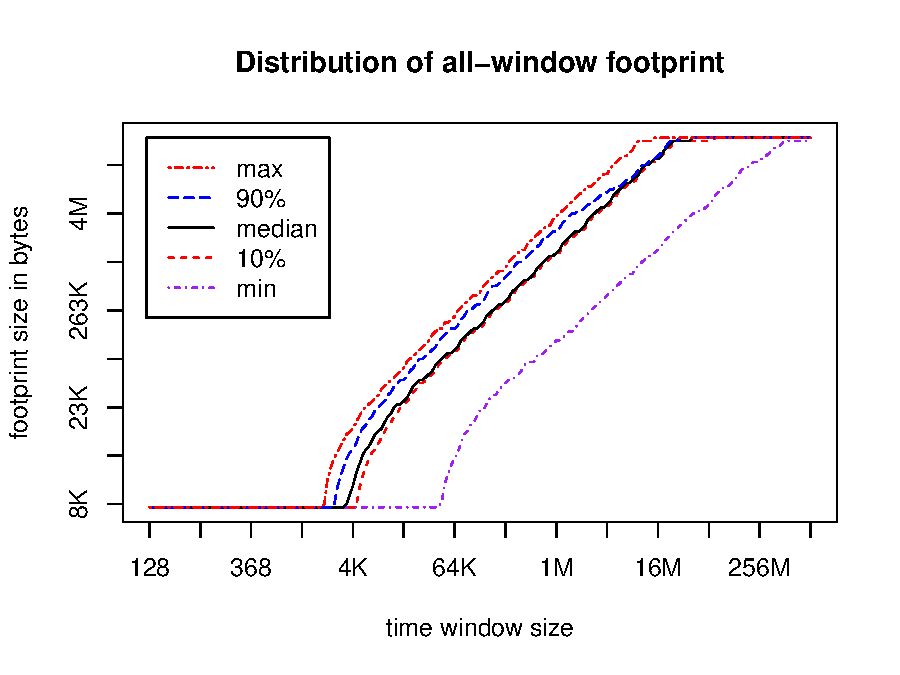
\includegraphics[width=\figwid]{figures/fp/183_equake_ref}
    \label{fp-equake-128}
  }\hfill \subfigure[{\bf Twolf} shows a narrow distribution ---80\%
  windows of the same length have nearly the same footprint. ]{
    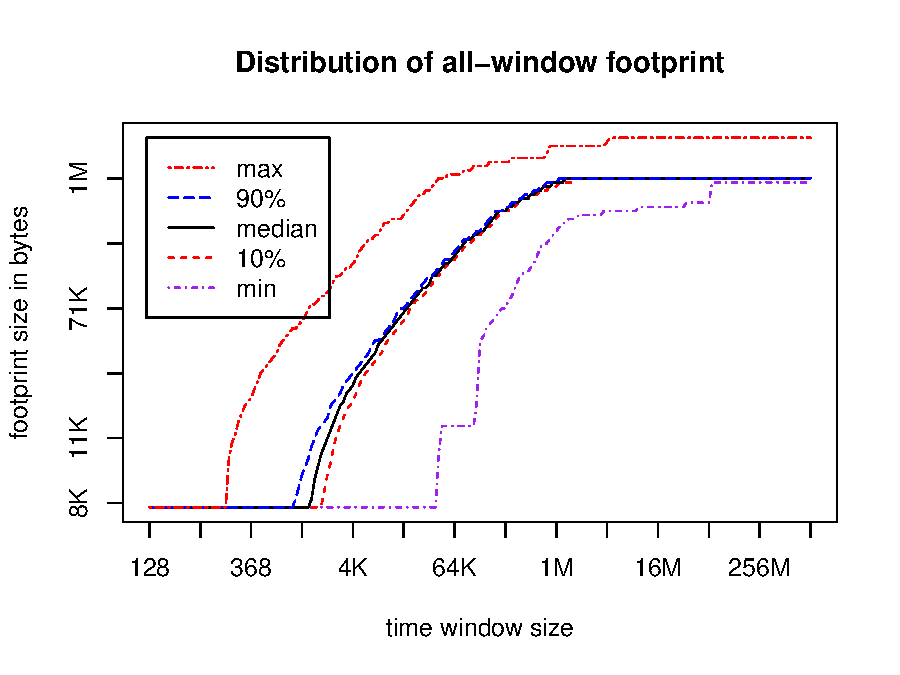
\includegraphics[width=\figwid]{figures/fp/300_twolf_ref}
    \label{fp-twolf-128}
  }\hfill
  \caption{The distribution of all-window footprint shows the
    characteristics of the working set in 4 SPEC2000 benchmarks.}
  \label{fig:all-fp-group}
\end{figure}

The footprint distribution shows highly summarized information about
program data usage.  For example, every point $<x,y>$ in the {\tt min} curve
shows the minimal footprint in all windows of size $x$ is $y$.  
As a sanity check, a reader can verify that the minimal and the
maximal footprints are monotone functions of the window size.  The
monotonicity should hold in theory but in an observation, it is not
guaranteed if we sample a set of windows rather than measure all
windows.

All-window footprint shows the characteristics of the working sets in
a program.  \emph{Gzip} has constant-size median working sets for
windows from 1 million to 256 million accesses, shown by
Figure~\ref{fp-gzip-128}.  In compression or decompression, the same
data buffers are repeatedly used for each chunk of the input or output
file.  Constant-size working sets are a result of complete data reuse.
\emph{Bzip2} creates larger auxiliary data structures in order to
improve compression ratio over a larger scope.  Its working sets
increase in size with the length of the execution window.  The rate of
increase, however, gradually decreases, as shown by
Figure~\ref{fp-bzip2-128}.

Shown in Figure~\ref{fp-equake-128}, {\tt Equake} has the clear
streaming access pattern because its working set size increases
linearly with the execution window length.  In fact, it shows the most
rapid growth, resulting in the largest footprint among all programs we
have tested.  90\% of footprints increase from 8KB to 8MB when window
size increases from 30K to 32M data accesses.  Its footprint
interferes with many other programs when running in shared cache.
{\tt Twolf} in Figure~\ref{fp-twolf-128} shows the smallest variation
in footprint size.  80\% of windows have nearly the
same size footprint.  These examples show that 
applications have different characteristics in their footprint distribution.

\paragraph{Measurement speed}
We have tested 12 SPEC2000 benchmark programs with the reference inputs. 
The length of the traces range from 4 billion to 108 billion, the size
of data ranges from 7 thousand to 787 thousand cache lines(64B), the number of
intervals ranges from 1.8 million to 48 billion, the average interval
length ranges from 504 to 19 thousand, and the measurement speed
ranges from 264 thousand data accesses per second to 8.4 million
accesses per second.  If we measure in terms of the number of windows
measured, the speed ranges from $10^{15}$ (a quadrillion) windows per
second to nearly $10^{18}$ (a quintillion) windows per second.

The speed closely correlates with the average interval length.  The
average length of $k$ means that in a random time window, 128 distinct
data elements are accessed by each $k$ accesses.  When the length is
500, the measurement speed is less than 300 thousand accesses per
second.  However, when the length is 19,000, the speed becomes 7.3
million accesses per second.  The average length is determined by the
length of the trace and the number of intervals.  Hence the cost of
the algorithm is determined by the number of intervals, $K$, more than
any other factor.

%to do: which input is used? test or ref? why it's said ref before and
%now it becomes test input
\paragraph{Comparison between CKlogM and NlogM}
The NlogM algorithm was the first to attempt complete all-window
measurement~\cite{DingC:PPOPP08}.  Here we compare NlogM with
CKlogM for $C=128$ and $C=256$.  Table~\ref{tbl:all-fp-time-compare} shows
the result of 14 SPEC2K benchmarks (that the NlogM method could finish
analyzing), including the length of the trace,
the size of data, the measurement time by NlogM, and the speedup
numbers by CKlogM for two Cs.  We have to use test inputs for comparison because it
takes too long for NlogM to measure larger inputs.  The measurement
time ranges from 414 seconds for \emph{mcf} to 4 hours
for \emph{parser} by NlogM and from 3 and 2 seconds for \emph{twolf}
to 18 and 17 minutes for \emph{ammp} by CKlogM when $C=128$ and
$C=256$.  The largest reduction is a factor of 316 for \emph{twolf}
from 10 minutes to 2 seconds.  The smallest reduction is a factor of 8
for \emph{mcf} from 7 minutes to 53 seconds. 

\begin{table}[h]
\small
\centering
\begin{tabular}{|l|c|c|c|c|c|c|c|}
\hline
prog. & $N$ & $M$ & NlogM & CKlogM C=128  & CKlogM C=256  \\ 
        &     &     & time[sec]  & time(speed) & time(speed) \\ \hline \hline
gzip    & 804M & 9K  & 12K   & 328(35)  & 246(47) \\ \hline
vpr     & 298M & 5K & 4K    & 84(49)  & 41(90) \\ \hline
gcc     & 255M & 15K  & 4K   & 37(102) & 19(198) \\ \hline
mesa    & 173M & 25K  & 2.6K  & 10(259) & 9(288) \\ \hline
art     & 1.0B  & 5K  & 12K   & 119(104) & 108(114) \\ \hline \hline
mcf     & 40M & 5K & 414   & 52(7.8) & 41(10) \\ \hline
equake  & 342M & 40K  & 5K    & 42(126) & 33(161) \\ \hline
crafty  & 935M & 8K & 15K   & 739(20)  & 187(78) \\ \hline
ammp    & 818M & 51K & 13K   & 1129(12)  & 1036(13) \\ \hline
parser  & 929M & 24K & 14K  & 142(101) & 98(147) \\ \hline \hline
gap     & 277M & 147K & 5K    & 30(168) & 20(252) \\ \hline
twolf   & 76M  & 309 & 631   & 3(210) & 2(316) \\ \hline \hline
median  & 320M & 12K & 5178 & 68({\bf 101}) & 41({\bf 131}) \\ \hline
mean    & 497M & 28K & 7343 & 226({\bf 100}) & 153({\bf 143}) \\ \hline
\end{tabular}
\caption{Time comparison for the test input of 12 SPEC 2K benchmarks.  On average, the measurement time is reduced from 2 hours per program to 73 and 52 seconds when $C=128$ and $256$ respectively. }
\label{tbl:all-fp-time-compare}
\end{table}

The average statistics is shown at the bottom of
Table~\ref{tbl:all-fp-time-compare}.  On average across 12 benchmarks, the
length of the trace is half billion memory accesses and the size of
data is 28 thousand words.  The average measurement time of NlogM is
two hours.  The average reduction by CKlogM is a factor of 100 to 73
seconds when $C=128$ and a factor of 142 to 52 seconds when $C=256$.
In other words, \emph{CKlogM reduces the average measurement time from
two hours to one minute.}

% Two programs, bzip2 and gzip, have different size footprints, which suggests that programs running with gzip have much less cache interference than when they are run with bzip.

\paragraph{Relation between $c$ and measurement speedup}
We define the \emph{speedup factor} by $\frac{N}{CK}$.  Intuitively, a
larger $c$ produces a greater speedup.  However, this is not true.  We
have measured all power-of-two $c$ values for all our tests and
studied the relation between $c$ and the potential speedup.  When the
speedup numbers for different $c$ were drawn as a curve, we have
observed variations in terms of whether a curve has a single peak or
whether the shape changes when a program is run with different inputs.
Figure~\ref{fig:ck-speedups} show the speedup factor for 4 programs whose
footprint we have shown in Figure~\ref{fig:all-fp-group}.  The highest
%speedup is in tens of thousands for {\em bzip2} a\cund {\em gzip}, one
speedup is in tens of thousands for {\tt bzip2} and {\tt gzip}, one
hundred thousand for {\tt equake}, and (too large to shown in the
figure) 1.6 million for {\tt twolf}.

\begin{figure}[h]
\centering
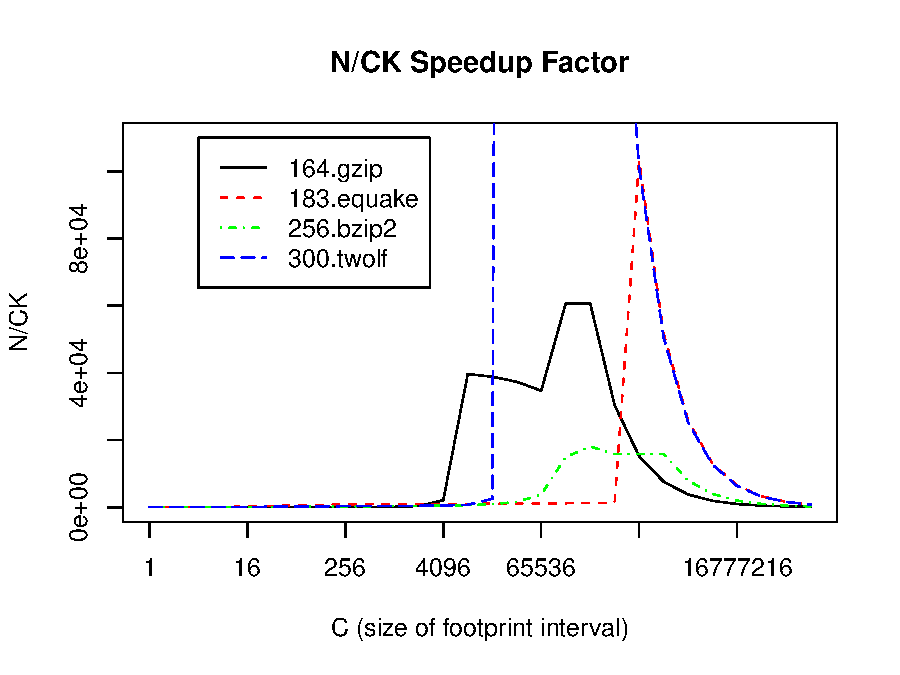
\includegraphics[width=0.7\textwidth]{figures/fp/ck}
\caption{$\frac{N}{CK}$ gives the speedup factors for 4 SPEC CPU2000
  benchmarks.  The speedup factors for {\tt twolf} are as high as 1.6
  million but are not shown above 100K in order to make other numbers
  easy to see.}
\label{fig:ck-speedups}
\end{figure}

\paragraph{Comparison with Miss Count}
It is interesting to consider the relation between the number of
misses in a window and the footprint of the window.  On average, the
number of misses is the miss rate times the window size.  Therefore,
the average miss count grows linearly.  It is unbounded if a program
executes forever.  The footprint is bounded by the size of program
data.  The growth cannot be always linear.

This difference is shown in the example of \emph{Gzip} result in
Figure~\ref{fig:miss-fp-comp}.  The miss count should be in the unit of
64-byte blocks.  The figure shows it in bytes growing linearly from
$2^{-9}$ byte to $2^{26}$ (83MB or 1.3 million misses) for window
sizes ranging from 1 access to 18 billion.  For the same window sizes,
the footprint grows from 64 bytes (1 block) to 83MB.  This difference
leads to different predictions of cache interference.  We compare
the accuracy of these predictions in cache sharing models, which will
be investigated in Chapter~\ref{chap:corun}.

\begin{figure}[h]
\centering
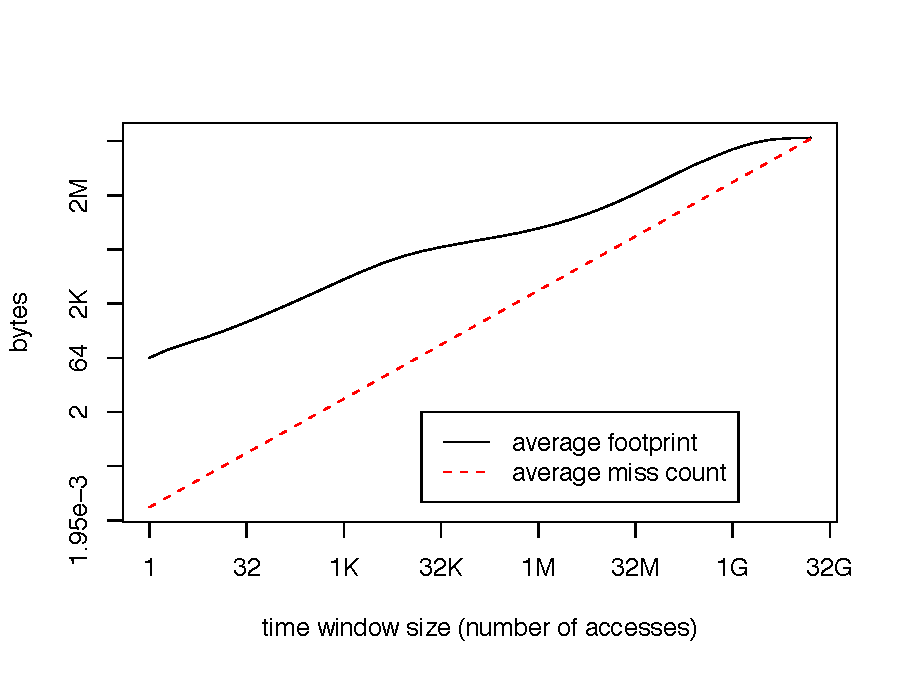
\includegraphics[width=0.7\textwidth]{figures/fp/miss_fp_comp}
\caption{Comparison of linear miss count growth and non-linear
  footprint growth in \emph{Gzip}.}
\label{fig:miss-fp-comp}
\end{figure}


\subsection{Efficiency of Average-footprint Analysis}
\label{subsec:fp-eval-aver-fp}
We have implemented the average-footprint analysis algorithm in a
Pin-based profiling tool
and tested 26 SPEC2K benchmarks, 12 integer and 14 floating-point,
and 29 SPEC2006 benchmarks, 12 integer and 17 floating-point. All
benchmarks are instrumented by Pin~\cite{Pin:PLDI05} and different
benchmarks are profiled on a linux cluster in parallel, with each node
has two 3.2GHz 64-bit Intel Xeon processors with 1MB L2 cache each and
6GB physical memory total.
\begin{comment}
a machine with an Intel Core i5-660 processor and 4GB physical
memory. The machine is installed with Fedora 13 and GCC 4.4.5.
\end{comment}

\paragraph{Average footprint overview}
Figure~\ref{fig:aver-fp-bzip2} shows an example average footprint
graph of bzip2 from SPEC2006 benchmark suite. The graph shows window
size, measured in number of data accesses with linear scale, in
$x$-axis and average footprint, measured in kilo-bytes, in the
$y$-axis. Since our measurements are based on 64-byte blocks, the
footprint sizes are always multiples of 64. At each window size, there
is one and only one average footprint value corresponding to the window
size. We connect all the average footprint points into a line, and
name the line {\em average footprint curve}. For each run of a
sequential program with a given input, only one average footprint curve
exists for this run.

\begin{figure}[!h]
  \centering
  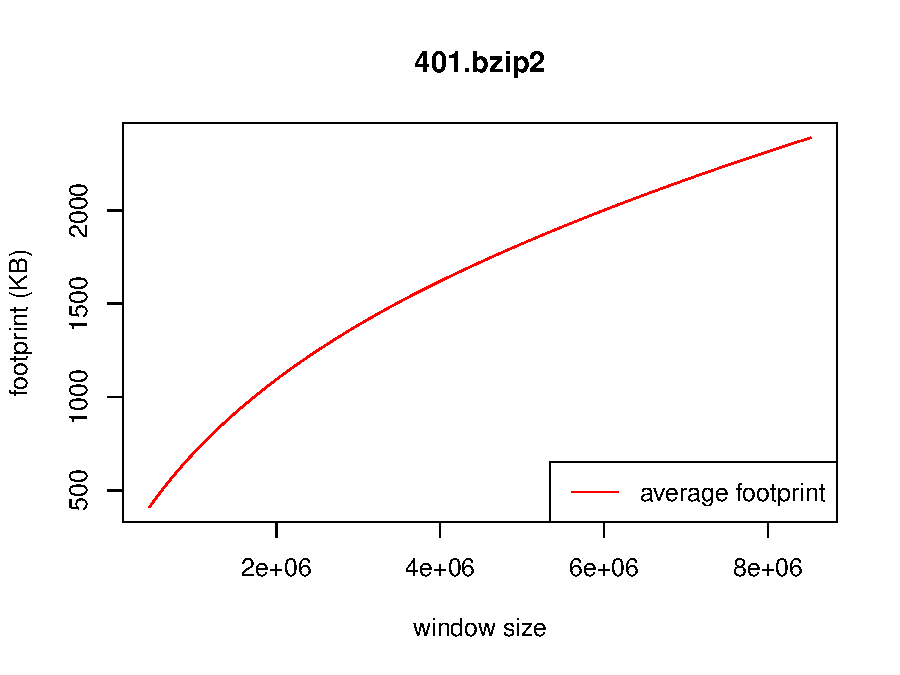
\includegraphics[width=0.7\textwidth]{figures/fp/401_bzip2_fp}
  \caption{The average footprint curve for SPEC20006/bzip2 with
    the first reference input.}
  \label{fig:aver-fp-bzip2}
\end{figure}

\paragraph{Measurement speed}
Table~\ref{tbl:aver-fp-speed} summarizes the analysis cost for the two
benchmark suites, and for each suite, the average for integer and for
floating-point programs.  It divides the 55 tests into four groups: 12
SPEC 2000 integer programs, 14 SPEC 2000 floating-point programs, 12
SPEC 2006 integer programs, and 17 SPEC 2006 floating-point programs.
The result of each group is summarized in three rows and three
columns.  The columns show the trace length, the data size, and the
slowdown ratio of the profiling time to the unmodified run time.  The
rows show the minimum, maximum, and the average slowdown factors for all benchmarks
of the group.

\begin{table*}[!h]
\centering
\small
\begin{tabular}{|c|c|c|c|c|}
\hline
benchmarks        &  stats     &trace length   &data size(64B lines)   &avg-FP slowdown(X) \\ \hline \hline
{\bf SPEC2000 INT}     & min   & 1.41 E+10     & 0.13 E+5      & 8.8 \\\cline{2-5}
    12  programs   & max   & 16.05 E+10    & 32.55 E+5     & 39.7 \\ \cline{2-5}
       & mean          & 7.52 E+10     & 11.67 E+5     & 28.8 \\ \hline \hline
{\bf SPEC2000 FP}      & min   & 3.03 E+10     & 0.56 E+5      & 9.7 \\ \cline{2-5}
    14   programs    & max   & 42.55 E+10    & 31.28 E+5     & 32.4 \\ \cline{2-5}
      & mean          & 17.44 E+10    & 14.16 E+5     & 21.9 \\ \hline \hline
{\bf SPEC2006 INT}     & min   & 4.88 E+10     & 3.01 E+5      & 8.1 \\ \cline{2-5}
     12  programs    & max   & 151.47 E+10   & 137.36 E+5    & 40.9 \\ \cline{2-5}
      & mean          & 47.20 E+10    & 34.05 E+5     & 20.7 \\ \hline \hline
{\bf SPEC2006 FP}      & min   & 20.73 E+10    & 0.40 E+5      & 9.4 \\ \cline{2-5}
      17   programs  & max   & 385.15 E+10   & 145.03 E+5    & 73.9 \\ \cline{2-5}
      & mean          & 138.85 E+10   & 58.69 E+5     & 26.1 \\ \hline
\end{tabular}
\caption{The min, max, and average costs (slowdowns) of average-footprint analysis for 55 SPEC 2000 and SPEC 2006 benchmark programs}
\label{tbl:aver-fp-speed}
\end{table*}

The minimum slowdowns in four benchmark groups are all below 10.  The
maximum slowdowns are 40, 32, 41, and 74.  The average slowdowns are between
21 in SPEC 2006 integer tests and 29 in SPEC 2000 integer tests.  On
average across all four groups, average-footprint analysis takes no more
than 30 times of the original execution time.

The individual results of the 29 SPEC2006  programs are not included in 
Table~\ref{tbl:all-times-spec2k} and Table~\ref{tbl:all-times-spec06}.
%Table~\ref{tbl:spec06-int-basic} and
%Table~\ref{tbl:spec06-fp-basic}. 
On average, an unmodified SPEC 2000 program (the original
program without any instrumentation or analysis) takes less than
3 minutes, and an unmodified SPEC 2006 program takes close to 10 minutes.
Average-footprint analysis takes 3 to 73 minutes for SPEC 2000
programs and 10 minutes (\emph{gcc}) to 10 hours (\emph{calculix}) 
for SPEC 2006 programs.


\paragraph{Comparison with All-footprint Analysis}

All-footprint analysis can analyze SPEC 2000 programs but not SPEC
2006 programs.  We compare average- and all-footprint analysis on SPEC
2000 programs in Table~\ref{tbl:all-aver-compare}. The table summarizes the
cost of the two analyses in these 15 tests in the last two columns.  The slowdowns by
average-footprint analysis are between 8.8 and 40.  The slowdowns by
all-footprint analysis are between 248 and 3160.  The average slowdown
is 40 for average-footprint analysis and about 1500 for all-footprint
analysis.  In other words, on average for these 15 programs,
average-footprint analysis is 38 times faster than all-footprint
analysis.

\begin{table*}[!h]
\small
\centering
\begin{tabular}{|c|c|c|c|c|c|c|c|c|c|c|}
\hline
{\bf 15 SPEC2000}       &trace length   &data size   &avg-FP &all-FP \\ 
{\bf Benchmarks}        &             &(Bytes)   &slowdown(X) &slowdown(X) \\ \hline \hline
min   & 1.41 E+10     & 1.98 E+6      & 8.8  & 248.2\\ \hline
max   & 16.05 E+10    & 2.08 E+8     & 39.7 & 3160.5\\ \hline
mean  & 8.20 E+10     & 6.43 E+7     & 26.1 & 1495.2\\ \hline 
\end{tabular}
\caption{Comparison of the min, max, and average slowdowns by average-footprint analysis and by all-footprint analysis.  On average, average-footprint analysis is 38 times faster.}
\label{tbl:all-aver-compare}
\end{table*}

All-footprint analysis takes too long for SPEC 2006 programs.  For
example, it takes average-footprint analysis 10 hours to profile
\emph{calculix}.  If all-footprint analysis is 38 times slower, it
would take more than two weeks to finish the same analysis.


\subsection{Efficiency of Footprint Sampling}
\label{sec:samp-result}

For this experiment, we choose somewhat arbitrarily the frequency
of one sample every 10 seconds.  The sample length depends on how
fast the footprint reaches cache size. 
In Table~\ref{tbl:sampling-fp-speed}, we 
show the slowdown of footprint sampling in the end-to-end run time by the
column marked $FP\-sampling\ slowdown$.  It ranges from 0\% to
2.14\%. Three programs have a visible cost of over 1\%.  They are
\emph{bwaves} 2.1\%, \emph{GemsFDTD} 1.3\% and \emph{milc} 1.5\%.  The
reason for the relatively high cost may be the non-trivial
interference between the sampling task and the parent task.  Across
all programs, the average visible overhead is below a half percent.
If we measure the total CPU time, sampling takes between 0\% and 80\%
of the original run time.  The average cost is 19\%, of which
over 18\% is hidden by shadow profiling.  The coverage is computed by the ratio of the number of
sampled instructions to the total number of instructions (counted by
our full trace profiling).  The coverage is as low as 0.006\% in
\emph{lbm}.

\begin{comment}
for calculation:
a = [4.2, 1.7, 0.2, 1.2, 0.9, 4.9, 7, 3, 2.6, 1.4, 14.4, 4.8, 3.8, 5.7, 20.6, 6.8, 6.8, 4.8, 9.5, 8.6, 3.3, 8.9]
\end{comment}

\begin{table}[!h]
\centering
\begin{tabular}{|c|c|c|c|c|c|}
\hline
{\bf 22 SPEC2006} &trace length &data size & FP-sampling & coverage \\ 
{\bf Benchmarks} &              &(bytes) & slowdown(\%) & (\%)\\\hline \hline
min & 0.2 E+11 & 0.3 E+7 & 0.00 & 0.01 \\ \hline
max & 20.6 E+11 & 175.7 E+7 & 2.14 & 3.1\\ \hline
mean & 5.69 E+11 & 36.96 E+7 & 0.47 & 0.94\\ \hline
\end{tabular}
\caption{Min, max, and average slowdowns by average-footprint sampling.  On average, sampling incurs only 0.47\% overhead.}
\label{tbl:sampling-fp-speed}
\end{table}


\section{Discussion}

We have presented the first accurate all-window footprint analysis,
CKlogM all-footprint analysis.
The new algorithm combines relative precision
approximation and trace compression to reduce the asymptotic cost to
$O(CKlogM)$.  We have successfully measured all-window footprints in
the SPEC2K benchmark suite in its full-length executions.  It is the
first time such complete measurement is made.  The results show that
applications differ in their footprints in terms of not just the size
but also the relation with time and the compactness of the
distribution.  The previous fastest accurate method, O(NlogM)
algorithm, could only measure these programs on their test input, for
which the new algorithm reduces the profiling time from 2 hours to 1
minute.  The all-window analysis measures a quadrillion to nearly a
quintillion footprints per second.

Although CKlogM algorithm have significantly reduced the measurement
time, the cost is still too high for real-size workloads. We
introduces a technique, average-footprint analysis, for measuring the
average footprint size. By confining the analysis to the average
rather than the full range, the 
problem  can be solved accurately by a linear-time algorithm.
The linear-time algorithm uses differential counting based on the
forward and backward reuse time distance.  When tested on SPEC CPU
2000 and 2006 benchmark suites, the average slowdowns are between 20
to 29, and the new linear-time algorithm is 38 times faster than
all-window footprint analysis. 

To make footprint an online measurable metric, we apply shadow
sampling to average-footprint analysis. Sampling reduces the visible
profiling overhead to around 0.47\%. While approximation and sampling
greatly reduce the profiling overhead, there is no guarantee that they
will preserve all the information. Whether the information captured is
representative of the whole program is the key to the usefulness of
all these techniques. We will evaluate all-footprint analysis,
average-footprint analysis, and shadow sampling in locality
models(Chapter~\ref{chap:model}) and cache sharing
models(Chapter~\ref{chap:corun}), and prove their contributions in real
use. 



\begin{table}[h]
\centering
\footnotesize
\begin{tabular}{|l|c|c|c|c|c|c|}
\hline
benchmark        &trace   &data size   &unmodified  &avg-FP &FP alg \\ 
&length &(64B lines) &time(sec) &time(sec) &cost(X)\\ \hline \hline
164.gzip         & 3.93 E+10     & 14.07 E+5     & 22.7          & 460.0         & 20.3 \\ \hline
175.vpr          & 6.26 E+10     & 0.38 E+5      & 33.7          & 809.0         & 24.0 \\ \hline
176.gcc          & 1.41 E+10     & 32.55 E+5     & 4.7   & 187.0         & 39.7 \\ \hline
181.mcf          & 2.29 E+10     & 12.62 E+5     & 46.6          & 408.0         & 8.8 \\ \hline
186.crafty       & 11.36 E+10    & 0.32 E+5      & 37.2          & 1427.0        & 38.4 \\ \hline
197.parser       & 16.05 E+10    & 4.11 E+5      & 80.2          & 1926.0        & 24.0 \\ \hline
252.eon          & 7.18 E+10     & 0.13 E+5      & 20.1          & 786.0         & 39.2 \\ \hline
253.perlbmk      & 4.69 E+10     & 18.14 E+5     & 14.9          & 542.0         & 36.3 \\ \hline
254.gap          & 11.16 E+10    & 31.50 E+5     & 39.4          & 1261.0        & 32.0 \\ \hline
255.vortex       & 6.45 E+10     & 10.92 E+5     & 19.7          & 770.0         & 39.0 \\ \hline
256.bzip2        & 4.72 E+10     & 14.71 E+5     & 23.4          & 548.0         & 23.4 \\ \hline
300.twolf        & 14.74 E+10    & 0.60 E+5      & 93.8          & 1917.0        & 20.4 \\ \hline
\hline
168.wupwise      & 15.68 E+10    & 28.82 E+5     & 112.8         & 1695.0        & 15.0 \\ \hline
171.swim         & 9.02 E+10     & 31.21 E+5     & 99.7          & 1141.0        & 11.4 \\ \hline
172.mgrid        & 42.55 E+10    & 9.10 E+5      & 175.2         & 4395.0        & 25.1 \\ \hline
173.applu        & 18.47 E+10    & 28.57 E+5     & 68.0          & 1999.0        & 29.4 \\ \hline
177.mesa         & 15.85 E+10    & 1.37 E+5      & 56.1          & 1799.0        & 32.1 \\ \hline
178.galgel       & 39.75 E+10    & 8.47 E+5      & 135.8         & 4397.0        & 32.4 \\ \hline
179.art          & 3.03 E+10     & 0.56 E+5      & 48.2          & 470.0         & 9.7 \\ \hline
183.equake       & 6.87 E+10     & 6.80 E+5      & 33.5          & 774.0         & 23.1 \\ \hline
187.facerec      & 14.62 E+10    & 2.98 E+5      & 63.7          & 1623.0        & 25.5 \\ \hline
188.ammp         & 14.26 E+10    & 2.14 E+5      & 84.4          & 1738.0        & 20.6 \\ \hline
189.lucas        & 15.07 E+10    & 25.95 E+5     & 63.9          & 1685.0        & 26.4 \\ \hline
191.fma3d        & 16.04 E+10    & 17.06 E+5     & 82.6          & 1854.0        & 22.4 \\ \hline
200.sixtrack     & 14.20 E+10    & 3.94 E+5      & 133.0         & 1608.0        & 12.1 \\ \hline
301.apsi         & 18.69 E+10    & 31.28 E+5     & 102.2         & 2218.0        & 21.7 \\ \hline
\end{tabular}
\caption{Individual statistics of the 26 SPEC2000 test programs}
\label{tbl:all-times-spec2k}
\end{table}

\begin{table}[h]
\centering
\footnotesize
\begin{tabular}{|l|c|c|c|c|c|c|}
\hline
benchmark        &trace   &data size   &unmodified  &avg-FP &FP alg \\ 
&length &(64B lines) &time(sec) &time(sec) &cost(X)\\ \hline \hline
400.perlbench    & 21.99 E+10    & 52.31 E+5     & 222.3         & 2478.0        & 11.1 \\ \hline
401.bzip2        & 9.73 E+10     & 11.98 E+5     & 129.4         & 1051.0        & 8.1 \\ \hline
403.gcc          & 4.88 E+10     & 41.74 E+5     & 31.5          & 594.0         & 18.8 \\ \hline
429.mcf          & 21.61 E+10    & 137.36 E+5    & 338.3         & 3627.0        & 10.7 \\ \hline
445.gobmk        & 12.48 E+10    & 3.06 E+5      & 67.0          & 1458.0        & 21.8 \\ \hline
456.hmmer        & 68.40 E+10    & 6.61 E+5      & 178.8         & 6441.0        & 36.0 \\ \hline
458.sjeng        & 110.99 E+10   & 28.56 E+5     & 518.8         & 12906.0       & 24.9 \\ \hline
462.libquantum   & 151.47 E+10   & 20.99 E+5     & 633.3         & 14930.0       & 23.6 \\ \hline
464.h264ref      & 41.10 E+10    & 3.01 E+5      & 99.5          & 4075.0        & 40.9 \\ \hline
471.omnetpp      & 40.77 E+10    & 16.44 E+5     & 422.2         & 5797.0        & 13.7 \\ \hline
473.astar        & 29.57 E+10    & 35.99 E+5     & 229.1         & 3396.0        & 14.8 \\ \hline
483.xalancbmk    & 53.38 E+10    & 50.50 E+5     & 297.9         & 6943.0        & 23.3 \\ \hline
\hline
410.bwaves       & 190.51 E+10   & 145.03 E+5    & 555.4         & 18551.0       & 33.4 \\ \hline
416.gamess       & 144.61 E+10   & 0.52 E+5      & 212.2         & 15682.0       & 73.9 \\ \hline
433.milc         & 51.48 E+10    & 113.33 E+5    & 565.8         & 5852.0        & 10.3 \\ \hline
434.zeusmp       & 85.62 E+10    & 81.21 E+5     & 593.1         & 9584.0        & 16.2 \\ \hline
435.gromacs      & 130.60 E+10   & 2.22 E+5      & 853.8         & 12883.0       & 15.1 \\ \hline
436.cactusADM    & 230.01 E+10   & 102.33 E+5    & 1297.5        & 24751.0       & 19.1 \\ \hline
437.leslie3d     & 112.12 E+10   & 20.18 E+5     & 578.2         & 11546.0       & 20.0 \\ \hline
444.namd         & 117.12 E+10   & 7.36 E+5      & 501.7         & 11799.0       & 23.5 \\ \hline
447.dealII       & 109.73 E+10   & 88.48 E+5     & 417.3         & 12542.0       & 30.1 \\ \hline
450.soplex       & 20.73 E+10    & 76.33 E+5     & 236.3         & 2219.0        & 9.4 \\ \hline
453.povray       & 67.91 E+10    & 0.40 E+5      & 227.9         & 7134.0        & 31.3 \\ \hline
454.calculix     & 385.15 E+10   & 27.92 E+5     & 755.2         & 36728.0       & 48.6 \\ \hline
459.GemsFDTD     & 155.60 E+10   & 136.10 E+5    & 714.4         & 15719.0       & 22.0 \\ \hline
465.tonto        & 146.23 E+10   & 6.45 E+5      & 640.1         & 15280.0       & 23.9 \\ \hline
470.lbm          & 79.73 E+10    & 67.03 E+5     & 430.8         & 8645.0        & 20.1 \\ \hline
481.wrf          & 200.09 E+10   & 116.40 E+5    & 866.4         & 21419.0       & 24.7 \\ \hline
482.sphinx3      & 133.24 E+10   & 6.43 E+5      & 679.6         & 14750.0       & 21.7 \\ \hline

%\hline
\end{tabular}
\caption{Individual statistics of the 29 SPEC2006 test programs}
\label{tbl:all-times-spec06}
\end{table}

\begin{comment}
\begin{table}
\centering
\begin{tabular}{|l|c|c|c|c|}
\hline
$bench name$ & $n$ $(10^{11})$ & $m$ $(10^7 bytes)$ & $T(sec)$ \\ \hline \hline 
400.perlbench & 4.2 & 24.4 & 457 \\ \hline
401.bzip2 & 1.7 & 39.3 & 263 \\ \hline
403.gcc & 0.2 & 40.4 & 72 \\ \hline
429.mcf & 1.2 & 175.7 & 1172 \\ \hline
445.gobmk & 0.9 & 2.7 & 173 \\ \hline
456.hmmer & 4.9 & 4.2 & 303 \\ \hline
458.sjeng & 7.0 & 18.2 & 1356 \\ \hline
462.libquantum & 3.0 & 16.8 & 1391 \\ \hline
464.h264ref & 2.6 & 2.7 & 143 \\ \hline
471.omnetpp & 2.3 & 17.6 & 1048 \\ \hline
473.astar & 1.4 & 29.5 & 512 \\ \hline
483.xalancbmk & 3.6 & 43.8 & 778 \\ \hline
\end{tabular} 
\caption{The SPEC2006 integer benchmarks. 
For each benchmark, $n$ is the memory trace length of whole execution, $m$ is 
the number of distinct data blocks (size in bytes) accessed during the execution, and $T$ is the
execution time without any instrumentation or analysis.}
\label{tbl:spec06-int-basic}
\end{table}

\begin{table}
\centering
\begin{tabular}{|l|c|c|c|c|}
\hline
$bench name$ & $n$ $(10^{11})$ & $m$ $(10^7 bytes)$& $T(sec)$ \\ \hline \hline 
410.bwaves & 14.4 & 98.2 & 1664 \\ \hline
416.gamess & 4.8 & 0.3 & 444 \\ \hline
433.milc & 3.8 & 74.2 & 1077 \\ \hline
434.zeusmp & 5.7 & 51.9 & 1555 \\ \hline
435.gromacs & 9.8 & 1.4 & 1272 \\ \hline
436.cactusADM & 20.6 & 65.5 & 3411 \\ \hline
437.leslie3d & 6.8 & 12.9 & 1212 \\ \hline
444.namd & 6.8 & 4.7 & 915 \\ \hline
447.dealII & 7.3 & 88.5 & 773 \\ \hline
450.soplex & 1.0 & 16.2 & 604 \\ \hline
453.povray & 4.8 & 0.3 & 493 \\ \hline
454.calculix & 9.5 & 16.4 & 1512 \\ \hline
459.GemsFDTD & 8.6 & 86.9 & 1397 \\ \hline
465.tonto & 10.0 & 5.2 & 1312 \\ \hline
470.lbm & 3.3 & 42.9 & 1491 \\ \hline
481.wrf & 9.7 & 76.8 & 1895 \\ \hline
482.sphinx3 & 8.9 & 5.1 & 1765 \\ \hline
\end{tabular} 
\caption{The SPEC2006 floating-point benchmarks. 
For each benchmark, $n$ is the memory trace length of whole execution, $m$ is 
the number of distinct data blocks (size in bytes) accessed during the execution, and $T$ is the
execution time without any instrumentation or analysis.}
\label{tbl:spec06-fp-basic}
\end{table}
\end{comment}

